%%%%%%%%%%%%%%%%%%%%%%%%%%%%%%%%%%%%%%%%%%%%%%%%%%%%%%%%%%%%%%%%%%%%%%%%%%%%%%%%%%%%%%%%%%%%%%%%%
%
% Document:      DM  product tree
%
%%%%%%%%%%%%%%%%%%%%%%%%%%%%%%%%%%%%%%%%%%%%%%%%%%%%%%%%%%%%%%%%%%%%%%%%%%%%%%
\documentclass{article}
\usepackage{times,layouts}
\usepackage{tikz,hyperref,amsmath}
\usetikzlibrary{positioning,arrows,shapes,decorations.shapes,shapes.arrows}
\usetikzlibrary{backgrounds,calc}
\usepackage[paperwidth=30cm,paperheight=165cm,
left=-2mm,top=3mm,bottom=0mm,right=0mm,
noheadfoot,marginparwidth=0pt,includemp=false,
textwidth=30cm,textheight=50mm]{geometry}
\newcommand\showpage{%
\setlayoutscale{0.5}\setlabelfont{\tiny}\printheadingsfalse\printparametersfalse
\currentpage\pagedesign}
\hypersetup{pdftitle={DM organisation }, pdfsubject={Diagram illustrating the
products in LSST DM }, pdfauthor={ William O'Mullane}}
\tikzstyle{wbbox}=[rectangle, rounded corners=3pt, draw=black, top color=blue!50!white, bottom color=white, very thick, minimum height=12mm, inner sep=2pt, text centered, text width=30mm] 
\tikzstyle{pbox}=[rectangle, rounded corners=3pt, draw=black, top color=yellow!50!white, bottom color=white, very thick, minimum height=22pt, inner sep=2pt, text centered, text width=35mm] 
\tikzstyle{pline}=[-, thick]\begin{document}
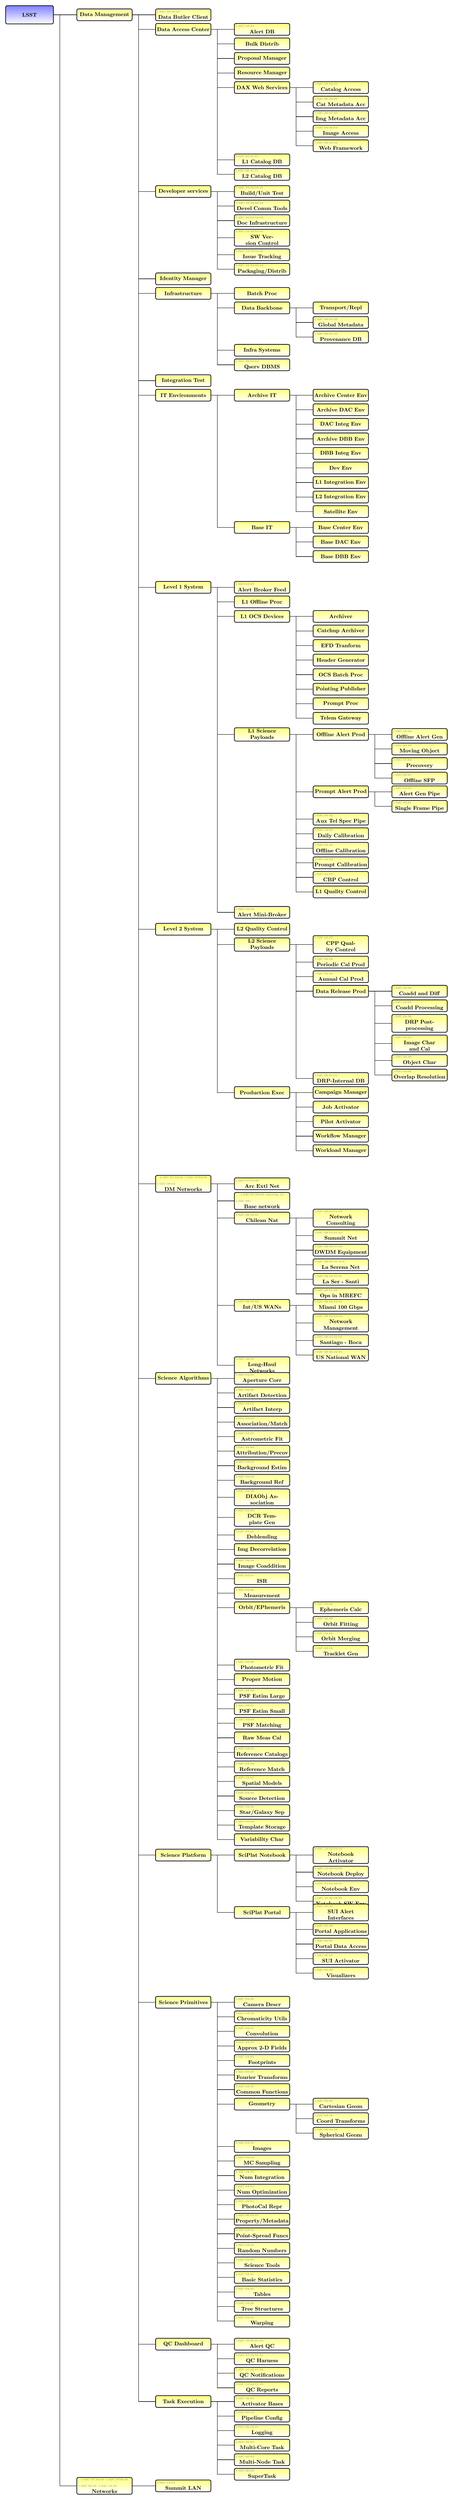
\begin{tikzpicture}[node distance=0mm]
\node (LSST) [wbbox]{\textbf{LSST}}; 
\node (DM) [pbox,right=15mm of LSST] {\textbf{Data Management}}; 
 \draw[pline] (LSST.east) -| ++(0.4,0)  |- (DM.west);
 \node (BUTLER) [pbox,right=15mm of DM] {{\tiny \color{gray}1.02C.06.02.01} \newline\textbf{Data Butler Client}}; 
 \draw[pline] (DM.east) -| ++(0.4,0)  |- (BUTLER.west);
 \node (DAC) [pbox,below=4pt of BUTLER] {\textbf{Data Access Center}}; 
 \draw[pline] (DM.east) -| ++(0.4,0)  |- (DAC.west);
 \node (ALERTDB) [pbox,right=15mm of DAC] {{\tiny \color{gray}1.02C.03.03} \newline\textbf{Alert DB}}; 
 \draw[pline] (DAC.east) -| ++(0.4,0)  |- (ALERTDB.west);
 \node (BULKD) [pbox,below=4pt of ALERTDB] {\textbf{Bulk Distrib}}; 
 \draw[pline] (DAC.east) -| ++(0.4,0)  |- (BULKD.west);
 \node (DACPROP) [pbox,below=4pt of BULKD] {\textbf{Proposal Manager}}; 
 \draw[pline] (DAC.east) -| ++(0.4,0)  |- (DACPROP.west);
 \node (DACRM) [pbox,below=4pt of DACPROP] {\textbf{Resource Manager}}; 
 \draw[pline] (DAC.east) -| ++(0.4,0)  |- (DACRM.west);
 \node (DAX) [pbox,below=4pt of DACRM] {\textbf{DAX Web Services}}; 
 \draw[pline] (DAC.east) -| ++(0.4,0)  |- (DAX.west);
 \node (DAXCAT) [pbox,right=15mm of DAX] {{\tiny \color{gray}1.02C.06.02.05} \newline\textbf{Catalog Access}}; 
 \draw[pline] (DAX.east) -| ++(0.4,0)  |- (DAXCAT.west);
 \node (DAXCMETA) [pbox,below=4pt of DAXCAT] {{\tiny \color{gray}1.02C.06.02.05} \newline\textbf{Cat Metadata Acc}}; 
 \draw[pline] (DAX.east) -| ++(0.4,0)  |- (DAXCMETA.west);
 \node (DAXIMETA) [pbox,below=4pt of DAXCMETA] {{\tiny \color{gray}1.02C.06.02.05} \newline\textbf{Img Metadata Acc}}; 
 \draw[pline] (DAX.east) -| ++(0.4,0)  |- (DAXIMETA.west);
 \node (DAXIMG) [pbox,below=4pt of DAXIMETA] {{\tiny \color{gray}1.02C.06.02.04} \newline\textbf{Image Access}}; 
 \draw[pline] (DAX.east) -| ++(0.4,0)  |- (DAXIMG.west);
 \node (DAXWEB) [pbox,below=4pt of DAXIMG] {{\tiny \color{gray}1.02C.06.02.02} \newline\textbf{Web Framework}}; 
 \draw[pline] (DAX.east) -| ++(0.4,0)  |- (DAXWEB.west);
 \node (L1DB) [pbox,below=112pt of DAX] {{\tiny \color{gray}1.02C.06.01.01} \newline\textbf{L1 Catalog DB}}; 
 \draw[pline] (DAC.east) -| ++(0.4,0)  |- (L1DB.west);
 \node (L2DB) [pbox,below=4pt of L1DB] {{\tiny \color{gray}1.02C.06.01.01} \newline\textbf{L2 Catalog DB}}; 
 \draw[pline] (DAC.east) -| ++(0.4,0)  |- (L2DB.west);
 \node (DEVEL) [pbox,below=280pt of DAC] {\textbf{Developer services}}; 
 \draw[pline] (DM.east) -| ++(0.4,0)  |- (DEVEL.west);
 \node (CI) [pbox,right=15mm of DEVEL] {{\tiny \color{gray}1.02C.10.02.03.01} \newline\textbf{Build/Unit Test}}; 
 \draw[pline] (DEVEL.east) -| ++(0.4,0)  |- (CI.west);
 \node (COMMS) [pbox,below=4pt of CI] {{\tiny \color{gray}1.02C.10.02.03.04} \newline\textbf{Devel Comm Tools}}; 
 \draw[pline] (DEVEL.east) -| ++(0.4,0)  |- (COMMS.west);
 \node (DOCS) [pbox,below=4pt of COMMS] {{\tiny \color{gray}1.02C.10.02.03.03} \newline\textbf{Doc Infrastructure}}; 
 \draw[pline] (DEVEL.east) -| ++(0.4,0)  |- (DOCS.west);
 \node (DVCS) [pbox,below=4pt of DOCS] {{\tiny \color{gray}1.02C.10.02.03.01} \newline\textbf{SW Version Control}}; 
 \draw[pline] (DEVEL.east) -| ++(0.4,0)  |- (DVCS.west);
 \node (ISSUE) [pbox,below=4pt of DVCS] {{\tiny \color{gray}1.02C.10.02.03.05} \newline\textbf{Issue Tracking}}; 
 \draw[pline] (DEVEL.east) -| ++(0.4,0)  |- (ISSUE.west);
 \node (PKG) [pbox,below=4pt of ISSUE] {{\tiny \color{gray}1.02C.10.02.03.02} \newline\textbf{Packaging/Distrib}}; 
 \draw[pline] (DEVEL.east) -| ++(0.4,0)  |- (PKG.west);
 \node (IDM) [pbox,below=140pt of DEVEL] {\textbf{Identity Manager}}; 
 \draw[pline] (DM.east) -| ++(0.4,0)  |- (IDM.west);
 \node (INFRA) [pbox,below=4pt of IDM] {\textbf{Infrastructure}}; 
 \draw[pline] (DM.east) -| ++(0.4,0)  |- (INFRA.west);
 \node (BPS) [pbox,right=15mm of INFRA] {\textbf{Batch Proc}}; 
 \draw[pline] (INFRA.east) -| ++(0.4,0)  |- (BPS.west);
 \node (DBB) [pbox,below=4pt of BPS] {\textbf{Data Backbone}}; 
 \draw[pline] (INFRA.east) -| ++(0.4,0)  |- (DBB.west);
 \node (DTR) [pbox,right=15mm of DBB] {\textbf{Transport/Repl}}; 
 \draw[pline] (DBB.east) -| ++(0.4,0)  |- (DTR.west);
 \node (GMDS) [pbox,below=4pt of DTR] {{\tiny \color{gray}1.02C.06.02.05} \newline\textbf{Global Metadata}}; 
 \draw[pline] (DBB.east) -| ++(0.4,0)  |- (GMDS.west);
 \node (PRVDB) [pbox,below=4pt of GMDS] {{\tiny \color{gray}1.02C.06.01.01} \newline\textbf{Provenance DB}}; 
 \draw[pline] (DBB.east) -| ++(0.4,0)  |- (PRVDB.west);
 \node (INFRASYS) [pbox,below=56pt of DBB] {\textbf{Infra Systems}}; 
 \draw[pline] (INFRA.east) -| ++(0.4,0)  |- (INFRASYS.west);
 \node (QSERV) [pbox,below=4pt of INFRASYS] {{\tiny \color{gray}1.02C.06.02.03} \newline\textbf{Qserv DBMS}}; 
 \draw[pline] (INFRA.east) -| ++(0.4,0)  |- (QSERV.west);
 \node (INTGTEST) [pbox,below=140pt of INFRA] {\textbf{Integration Test}}; 
 \draw[pline] (DM.east) -| ++(0.4,0)  |- (INTGTEST.west);
 \node (ITENV) [pbox,below=4pt of INTGTEST] {\textbf{IT Environments}}; 
 \draw[pline] (DM.east) -| ++(0.4,0)  |- (ITENV.west);
 \node (ITARC) [pbox,right=15mm of ITENV] {\textbf{Archive IT}}; 
 \draw[pline] (ITENV.east) -| ++(0.4,0)  |- (ITARC.west);
 \node (CTRENV) [pbox,right=15mm of ITARC] {\textbf{Archive Center Env}}; 
 \draw[pline] (ITARC.east) -| ++(0.4,0)  |- (CTRENV.west);
 \node (DACENV) [pbox,below=4pt of CTRENV] {\textbf{Archive DAC Env}}; 
 \draw[pline] (ITARC.east) -| ++(0.4,0)  |- (DACENV.west);
 \node (DACINTGR) [pbox,below=4pt of DACENV] {\textbf{DAC Integ Env}}; 
 \draw[pline] (ITARC.east) -| ++(0.4,0)  |- (DACINTGR.west);
 \node (DBBENV) [pbox,below=4pt of DACINTGR] {\textbf{Archive DBB Env}}; 
 \draw[pline] (ITARC.east) -| ++(0.4,0)  |- (DBBENV.west);
 \node (DBBINTGR) [pbox,below=4pt of DBBENV] {\textbf{DBB Integ Env}}; 
 \draw[pline] (ITARC.east) -| ++(0.4,0)  |- (DBBINTGR.west);
 \node (DEVENV) [pbox,below=4pt of DBBINTGR] {\textbf{Dev Env}}; 
 \draw[pline] (ITARC.east) -| ++(0.4,0)  |- (DEVENV.west);
 \node (L1INTGR) [pbox,below=4pt of DEVENV] {\textbf{L1 Integration Env}}; 
 \draw[pline] (ITARC.east) -| ++(0.4,0)  |- (L1INTGR.west);
 \node (L2INTGR) [pbox,below=4pt of L1INTGR] {\textbf{L2 Integration Env}}; 
 \draw[pline] (ITARC.east) -| ++(0.4,0)  |- (L2INTGR.west);
 \node (SATENV) [pbox,below=4pt of L2INTGR] {\textbf{Satellite Env}}; 
 \draw[pline] (ITARC.east) -| ++(0.4,0)  |- (SATENV.west);
 \node (ITBASE) [pbox,below=224pt of ITARC] {\textbf{Base IT}}; 
 \draw[pline] (ITENV.east) -| ++(0.4,0)  |- (ITBASE.west);
 \node (BCTRENV) [pbox,right=15mm of ITBASE] {\textbf{Base Center Env}}; 
 \draw[pline] (ITBASE.east) -| ++(0.4,0)  |- (BCTRENV.west);
 \node (BDACENV) [pbox,below=4pt of BCTRENV] {\textbf{Base DAC Env}}; 
 \draw[pline] (ITBASE.east) -| ++(0.4,0)  |- (BDACENV.west);
 \node (BDBBENV) [pbox,below=4pt of BDACENV] {\textbf{Base DBB Env}}; 
 \draw[pline] (ITBASE.east) -| ++(0.4,0)  |- (BDBBENV.west);
 \node (L1) [pbox,below=336pt of ITENV] {\textbf{Level 1 System}}; 
 \draw[pline] (DM.east) -| ++(0.4,0)  |- (L1.west);
 \node (BRKRFEED) [pbox,right=15mm of L1] {{\tiny \color{gray}1.02C.03.03} \newline\textbf{Alert Broker Feed}}; 
 \draw[pline] (L1.east) -| ++(0.4,0)  |- (BRKRFEED.west);
 \node (L1OFFL) [pbox,below=4pt of BRKRFEED] {\textbf{L1 Offline Proc}}; 
 \draw[pline] (L1.east) -| ++(0.4,0)  |- (L1OFFL.west);
 \node (L1ONL) [pbox,below=4pt of L1OFFL] {\textbf{L1 OCS Devices}}; 
 \draw[pline] (L1.east) -| ++(0.4,0)  |- (L1ONL.west);
 \node (ARC) [pbox,right=15mm of L1ONL] {\textbf{Archiver}}; 
 \draw[pline] (L1ONL.east) -| ++(0.4,0)  |- (ARC.west);
 \node (CARC) [pbox,below=4pt of ARC] {\textbf{Catchup Archiver}}; 
 \draw[pline] (L1ONL.east) -| ++(0.4,0)  |- (CARC.west);
 \node (EFDT) [pbox,below=4pt of CARC] {\textbf{EFD Tranform}}; 
 \draw[pline] (L1ONL.east) -| ++(0.4,0)  |- (EFDT.west);
 \node (HEADER) [pbox,below=4pt of EFDT] {\textbf{Header Generator}}; 
 \draw[pline] (L1ONL.east) -| ++(0.4,0)  |- (HEADER.west);
 \node (OCSBAT) [pbox,below=4pt of HEADER] {\textbf{OCS Batch Proc}}; 
 \draw[pline] (L1ONL.east) -| ++(0.4,0)  |- (OCSBAT.west);
 \node (POINTP) [pbox,below=4pt of OCSBAT] {\textbf{Pointing Publisher}}; 
 \draw[pline] (L1ONL.east) -| ++(0.4,0)  |- (POINTP.west);
 \node (PRMPT) [pbox,below=4pt of POINTP] {\textbf{Prompt Proc}}; 
 \draw[pline] (L1ONL.east) -| ++(0.4,0)  |- (PRMPT.west);
 \node (TMG) [pbox,below=4pt of PRMPT] {\textbf{Telem Gateway}}; 
 \draw[pline] (L1ONL.east) -| ++(0.4,0)  |- (TMG.west);
 \node (L1SCI) [pbox,below=196pt of L1ONL] {\textbf{L1 Science Payloads}}; 
 \draw[pline] (L1.east) -| ++(0.4,0)  |- (L1SCI.west);
 \node (APOFFL) [pbox,right=15mm of L1SCI] {\textbf{Offline Alert Prod}}; 
 \draw[pline] (L1SCI.east) -| ++(0.4,0)  |- (APOFFL.west);
 \node (ALRTOFFL) [pbox,right=15mm of APOFFL] {{\tiny \color{gray}1.02C.03.03} \newline\textbf{Offline Alert Gen}}; 
 \draw[pline] (APOFFL.east) -| ++(0.4,0)  |- (ALRTOFFL.west);
 \node (MOPS) [pbox,below=4pt of ALRTOFFL] {{\tiny \color{gray}1.02C.03.06} \newline\textbf{Moving Object}}; 
 \draw[pline] (APOFFL.east) -| ++(0.4,0)  |- (MOPS.west);
 \node (PRECOV) [pbox,below=4pt of MOPS] {{\tiny \color{gray}1.02C.03.04} \newline\textbf{Precovery}}; 
 \draw[pline] (APOFFL.east) -| ++(0.4,0)  |- (PRECOV.west);
 \node (SFPOFFL) [pbox,below=4pt of PRECOV] {{\tiny \color{gray}1.02C.03.01} \newline\textbf{Offline SFP}}; 
 \draw[pline] (APOFFL.east) -| ++(0.4,0)  |- (SFPOFFL.west);
 \node (APPRMPT) [pbox,below=84pt of APOFFL] {\textbf{Prompt Alert Prod}}; 
 \draw[pline] (L1SCI.east) -| ++(0.4,0)  |- (APPRMPT.west);
 \node (ALERTPIPE) [pbox,right=15mm of APPRMPT] {{\tiny \color{gray}1.02C.03.03} \newline\textbf{Alert Gen Pipe}}; 
 \draw[pline] (APPRMPT.east) -| ++(0.4,0)  |- (ALERTPIPE.west);
 \node (SFPPIPE) [pbox,below=4pt of ALERTPIPE] {{\tiny \color{gray}1.02C.03.01} \newline\textbf{Single Frame Pipe}}; 
 \draw[pline] (APPRMPT.east) -| ++(0.4,0)  |- (SFPPIPE.west);
 \node (AUXTEL) [pbox,below=28pt of APPRMPT] {{\tiny \color{gray}1.02C.04.02} \newline\textbf{Aux Tel Spec Pipe}}; 
 \draw[pline] (L1SCI.east) -| ++(0.4,0)  |- (AUXTEL.west);
 \node (CALDAILY) [pbox,below=4pt of AUXTEL] {{\tiny \color{gray}1.02C.04.02} \newline\textbf{Daily Calibration}}; 
 \draw[pline] (L1SCI.east) -| ++(0.4,0)  |- (CALDAILY.west);
 \node (CALOFFL) [pbox,below=4pt of CALDAILY] {{\tiny \color{gray}1.02C.04.02} \newline\textbf{Offline Calibration}}; 
 \draw[pline] (L1SCI.east) -| ++(0.4,0)  |- (CALOFFL.west);
 \node (CALPRMPT) [pbox,below=4pt of CALOFFL] {{\tiny \color{gray}1.02C.04.02} \newline\textbf{Prompt Calibration}}; 
 \draw[pline] (L1SCI.east) -| ++(0.4,0)  |- (CALPRMPT.west);
 \node (CBPCTRL) [pbox,below=4pt of CALPRMPT] {{\tiny \color{gray}1.02C.04.02} \newline\textbf{CBP Control}}; 
 \draw[pline] (L1SCI.east) -| ++(0.4,0)  |- (CBPCTRL.west);
 \node (L1QC) [pbox,below=4pt of CBPCTRL] {\textbf{L1 Quality Control}}; 
 \draw[pline] (L1SCI.east) -| ++(0.4,0)  |- (L1QC.west);
 \node (MINIBRKR) [pbox,below=308pt of L1SCI] {{\tiny \color{gray}1.02C.03.03} \newline\textbf{Alert Mini-Broker}}; 
 \draw[pline] (L1.east) -| ++(0.4,0)  |- (MINIBRKR.west);
 \node (L2) [pbox,below=616pt of L1] {\textbf{Level 2 System}}; 
 \draw[pline] (DM.east) -| ++(0.4,0)  |- (L2.west);
 \node (L2QC) [pbox,right=15mm of L2] {\textbf{L2 Quality Control}}; 
 \draw[pline] (L2.east) -| ++(0.4,0)  |- (L2QC.west);
 \node (L2SCI) [pbox,below=4pt of L2QC] {\textbf{L2 Science Payloads}}; 
 \draw[pline] (L2.east) -| ++(0.4,0)  |- (L2SCI.west);
 \node (CPPQC) [pbox,right=15mm of L2SCI] {{\tiny \color{gray}1.02C.04.02} \newline\textbf{CPP Quality Control}}; 
 \draw[pline] (L2SCI.east) -| ++(0.4,0)  |- (CPPQC.west);
 \node (CPPSLOW) [pbox,below=4pt of CPPQC] {{\tiny \color{gray}1.02C.04.02} \newline\textbf{Periodic Cal Prod}}; 
 \draw[pline] (L2SCI.east) -| ++(0.4,0)  |- (CPPSLOW.west);
 \node (CPPYEAR) [pbox,below=4pt of CPPSLOW] {{\tiny \color{gray}1.02C.04.02} \newline\textbf{Annual Cal Prod}}; 
 \draw[pline] (L2SCI.east) -| ++(0.4,0)  |- (CPPYEAR.west);
 \node (DRP) [pbox,below=4pt of CPPYEAR] {\textbf{Data Release Prod}}; 
 \draw[pline] (L2SCI.east) -| ++(0.4,0)  |- (DRP.west);
 \node (COADPIPE) [pbox,right=15mm of DRP] {{\tiny \color{gray}1.02C.04.04} \newline\textbf{Coadd and Diff}}; 
 \draw[pline] (DRP.east) -| ++(0.4,0)  |- (COADPIPE.west);
 \node (COADPROC) [pbox,below=4pt of COADPIPE] {{\tiny \color{gray}1.02C.04.05} \newline\textbf{Coadd Processing}}; 
 \draw[pline] (DRP.east) -| ++(0.4,0)  |- (COADPROC.west);
 \node (DRPPOST) [pbox,below=4pt of COADPROC] {{\tiny \color{gray}1.02C.04.06} \newline\textbf{DRP Postprocessing}}; 
 \draw[pline] (DRP.east) -| ++(0.4,0)  |- (DRPPOST.west);
 \node (IMGCHAR) [pbox,below=4pt of DRPPOST] {{\tiny \color{gray}1.02C.04.03} \newline\textbf{Image Char and Cal}}; 
 \draw[pline] (DRP.east) -| ++(0.4,0)  |- (IMGCHAR.west);
 \node (MULTIFIT) [pbox,below=4pt of IMGCHAR] {{\tiny \color{gray}1.02C.04.06} \newline\textbf{Object Char}}; 
 \draw[pline] (DRP.east) -| ++(0.4,0)  |- (MULTIFIT.west);
 \node (OVERLAP) [pbox,below=4pt of MULTIFIT] {{\tiny \color{gray}1.02C.04.05} \newline\textbf{Overlap Resolution}}; 
 \draw[pline] (DRP.east) -| ++(0.4,0)  |- (OVERLAP.west);
 \node (DRPDB) [pbox,below=140pt of DRP] {{\tiny \color{gray}1.02C.06.01.01} \newline\textbf{DRP-Internal DB}}; 
 \draw[pline] (L2SCI.east) -| ++(0.4,0)  |- (DRPDB.west);
 \node (PRODEX) [pbox,below=252pt of L2SCI] {\textbf{Production Exec}}; 
 \draw[pline] (L2.east) -| ++(0.4,0)  |- (PRODEX.west);
 \node (CMPGN) [pbox,right=15mm of PRODEX] {\textbf{Campaign Manager}}; 
 \draw[pline] (PRODEX.east) -| ++(0.4,0)  |- (CMPGN.west);
 \node (JOBACTIV) [pbox,below=4pt of CMPGN] {\textbf{Job Activator}}; 
 \draw[pline] (PRODEX.east) -| ++(0.4,0)  |- (JOBACTIV.west);
 \node (PLTACTIV) [pbox,below=4pt of JOBACTIV] {\textbf{Pilot Activator}}; 
 \draw[pline] (PRODEX.east) -| ++(0.4,0)  |- (PLTACTIV.west);
 \node (WFM) [pbox,below=4pt of PLTACTIV] {\textbf{Workflow Manager}}; 
 \draw[pline] (PRODEX.east) -| ++(0.4,0)  |- (WFM.west);
 \node (WLM) [pbox,below=4pt of WFM] {\textbf{Workload Manager}}; 
 \draw[pline] (PRODEX.east) -| ++(0.4,0)  |- (WLM.west);
 \node (NETDM) [pbox,below=448pt of L2] {{\tiny \color{gray}1.02C.07.04.03 1.02C.0704.06 1.02C.08.03 } \newline\textbf{DM Networks}}; 
 \draw[pline] (DM.east) -| ++(0.4,0)  |- (NETDM.west);
 \node (NETARCH) [pbox,right=15mm of NETDM] {{\tiny \color{gray}1.02C.07.04.06} \newline\textbf{Arc Extl Net}}; 
 \draw[pline] (NETDM.east) -| ++(0.4,0)  |- (NETARCH.west);
 \node (NETBASE) [pbox,below=4pt of NETARCH] {{\tiny \color{gray}1.02C.07.04.03 (moving to 1.02C.08)} \newline\textbf{Base network}}; 
 \draw[pline] (NETDM.east) -| ++(0.4,0)  |- (NETBASE.west);
 \node (NETCHILE) [pbox,below=4pt of NETBASE] {{\tiny \color{gray}1.02C.08.03.01} \newline\textbf{Chilean Nat}}; 
 \draw[pline] (NETDM.east) -| ++(0.4,0)  |- (NETCHILE.west);
 \node (NETCONS) [pbox,right=15mm of NETCHILE] {{\tiny \color{gray}1.02C.08.03.01.02} \newline\textbf{Network Consulting}}; 
 \draw[pline] (NETCHILE.east) -| ++(0.4,0)  |- (NETCONS.west);
 \node (NETCPAG) [pbox,below=4pt of NETCONS] {{\tiny \color{gray}1.02C.08.03.01.03} \newline\textbf{Summit Net}}; 
 \draw[pline] (NETCHILE.east) -| ++(0.4,0)  |- (NETCPAG.west);
 \node (NETDWDM) [pbox,below=4pt of NETCPAG] {{\tiny \color{gray}1.02C.08.03.01.04} \newline\textbf{DWDM Equipment}}; 
 \draw[pline] (NETCHILE.east) -| ++(0.4,0)  |- (NETDWDM.west);
 \node (NETLSAG) [pbox,below=4pt of NETDWDM] {{\tiny \color{gray}1.02C.08.03.01.01A} \newline\textbf{La Serena Net}}; 
 \draw[pline] (NETCHILE.east) -| ++(0.4,0)  |- (NETLSAG.west);
 \node (NETLSSCL) [pbox,below=4pt of NETLSAG] {{\tiny \color{gray}1.02C.08.03.01.01} \newline\textbf{La Ser - Santi }}; 
 \draw[pline] (NETCHILE.east) -| ++(0.4,0)  |- (NETLSSCL.west);
 \node (NETOPTG) [pbox,below=4pt of NETLSSCL] {{\tiny \color{gray}1.02C.08.03.05} \newline\textbf{Ops in MREFC}}; 
 \draw[pline] (NETCHILE.east) -| ++(0.4,0)  |- (NETOPTG.west);
 \node (NETINTLUS) [pbox,below=140pt of NETCHILE] {{\tiny \color{gray}1.02C.08.03.02} \newline\textbf{Int/US WANs}}; 
 \draw[pline] (NETDM.east) -| ++(0.4,0)  |- (NETINTLUS.west);
 \node (NET100G) [pbox,right=15mm of NETINTLUS] {{\tiny \color{gray}1.02C.08.03.02.01} \newline\textbf{Miami 100 Gbps }}; 
 \draw[pline] (NETINTLUS.east) -| ++(0.4,0)  |- (NET100G.west);
 \node (NETMGT) [pbox,below=4pt of NET100G] {{\tiny \color{gray}1.02C.08.03.02.02} \newline\textbf{Network Management}}; 
 \draw[pline] (NETINTLUS.east) -| ++(0.4,0)  |- (NETMGT.west);
 \node (NETSPEC) [pbox,below=4pt of NETMGT] {{\tiny \color{gray}1.02C.08.03.02.03} \newline\textbf{Santiago - Boca }}; 
 \draw[pline] (NETINTLUS.east) -| ++(0.4,0)  |- (NETSPEC.west);
 \node (NETUSW) [pbox,below=4pt of NETSPEC] {{\tiny \color{gray}1.02C.08.03.02.01} \newline\textbf{US National WAN}}; 
 \draw[pline] (NETINTLUS.east) -| ++(0.4,0)  |- (NETUSW.west);
 \node (NETLHN) [pbox,below=84pt of NETINTLUS] {{\tiny \color{gray}1.02C.08.03} \newline\textbf{Long-Haul Networks}}; 
 \draw[pline] (NETDM.east) -| ++(0.4,0)  |- (NETLHN.west);
 \node (SCIALG) [pbox,below=336pt of NETDM] {\textbf{Science Algorithms}}; 
 \draw[pline] (DM.east) -| ++(0.4,0)  |- (SCIALG.west);
 \node (APCORR) [pbox,right=15mm of SCIALG] {{\tiny \color{gray}1.02C.04.05} \newline\textbf{Aperture Corr}}; 
 \draw[pline] (SCIALG.east) -| ++(0.4,0)  |- (APCORR.west);
 \node (ARTFDET) [pbox,below=4pt of APCORR] {{\tiny \color{gray}1.02C.03.01} \newline\textbf{Artifact Detection}}; 
 \draw[pline] (SCIALG.east) -| ++(0.4,0)  |- (ARTFDET.west);
 \node (ARTFINTP) [pbox,below=4pt of ARTFDET] {{\tiny \color{gray}1.02C.03.01} \newline\textbf{Artifact Interp}}; 
 \draw[pline] (SCIALG.east) -| ++(0.4,0)  |- (ARTFINTP.west);
 \node (ASSOC) [pbox,below=4pt of ARTFINTP] {{\tiny \color{gray}1.02C.04.05} \newline\textbf{Association/Match}}; 
 \draw[pline] (SCIALG.east) -| ++(0.4,0)  |- (ASSOC.west);
 \node (ASTROM) [pbox,below=4pt of ASSOC] {{\tiny \color{gray}1.02C.03.07} \newline\textbf{Astrometric Fit}}; 
 \draw[pline] (SCIALG.east) -| ++(0.4,0)  |- (ASTROM.west);
 \node (ATTRIB) [pbox,below=4pt of ASTROM] {{\tiny \color{gray}1.02C.03.06} \newline\textbf{Attribution/Precov}}; 
 \draw[pline] (SCIALG.east) -| ++(0.4,0)  |- (ATTRIB.west);
 \node (BKGDEST) [pbox,below=4pt of ATTRIB] {{\tiny \color{gray}1.02C.04.03} \newline\textbf{Background Estim}}; 
 \draw[pline] (SCIALG.east) -| ++(0.4,0)  |- (BKGDEST.west);
 \node (BKGDREF) [pbox,below=4pt of BKGDEST] {{\tiny \color{gray}1.02C.04.03} \newline\textbf{Background Ref}}; 
 \draw[pline] (SCIALG.east) -| ++(0.4,0)  |- (BKGDREF.west);
 \node (DASSOC) [pbox,below=4pt of BKGDREF] {{\tiny \color{gray}1.02C.03.02} \newline\textbf{DIAObj Association}}; 
 \draw[pline] (SCIALG.east) -| ++(0.4,0)  |- (DASSOC.west);
 \node (DCRTMPL) [pbox,below=4pt of DASSOC] {{\tiny \color{gray}1.02C.03.04} \newline\textbf{DCR Template Gen}}; 
 \draw[pline] (SCIALG.east) -| ++(0.4,0)  |- (DCRTMPL.west);
 \node (DEBLEND) [pbox,below=4pt of DCRTMPL] {{\tiny \color{gray}1.02C.04.05} \newline\textbf{Deblending}}; 
 \draw[pline] (SCIALG.east) -| ++(0.4,0)  |- (DEBLEND.west);
 \node (DECORR) [pbox,below=4pt of DEBLEND] {\textbf{Img Decorrelation}}; 
 \draw[pline] (SCIALG.east) -| ++(0.4,0)  |- (DECORR.west);
 \node (IMCOADD) [pbox,below=4pt of DECORR] {{\tiny \color{gray}1.02C.04.04} \newline\textbf{Image Coaddition}}; 
 \draw[pline] (SCIALG.east) -| ++(0.4,0)  |- (IMCOADD.west);
 \node (ISR) [pbox,below=4pt of IMCOADD] {{\tiny \color{gray}1.02C.03.01} \newline\textbf{ISR}}; 
 \draw[pline] (SCIALG.east) -| ++(0.4,0)  |- (ISR.west);
 \node (MEASURE) [pbox,below=4pt of ISR] {{\tiny \color{gray}1.02C.04.05} \newline\textbf{Measurement}}; 
 \draw[pline] (SCIALG.east) -| ++(0.4,0)  |- (MEASURE.west);
 \node (ORBEP) [pbox,below=4pt of MEASURE] {\textbf{Orbit/EPhemeris}}; 
 \draw[pline] (SCIALG.east) -| ++(0.4,0)  |- (ORBEP.west);
 \node (EPHEM) [pbox,right=15mm of ORBEP] {{\tiny \color{gray}1.02C.03.06} \newline\textbf{Ephemeris Calc}}; 
 \draw[pline] (ORBEP.east) -| ++(0.4,0)  |- (EPHEM.west);
 \node (ORBFIT) [pbox,below=4pt of EPHEM] {{\tiny \color{gray}1.02C.03.06} \newline\textbf{Orbit Fitting}}; 
 \draw[pline] (ORBEP.east) -| ++(0.4,0)  |- (ORBFIT.west);
 \node (ORBMERGE) [pbox,below=4pt of ORBFIT] {{\tiny \color{gray}1.02C.03.06} \newline\textbf{Orbit Merging}}; 
 \draw[pline] (ORBEP.east) -| ++(0.4,0)  |- (ORBMERGE.west);
 \node (TRACKLET) [pbox,below=4pt of ORBMERGE] {{\tiny \color{gray}1.02C.03.06} \newline\textbf{Tracklet Gen}}; 
 \draw[pline] (ORBEP.east) -| ++(0.4,0)  |- (TRACKLET.west);
 \node (PHOTOM) [pbox,below=84pt of ORBEP] {{\tiny \color{gray}1.02C.03.08} \newline\textbf{Photometric Fit}}; 
 \draw[pline] (SCIALG.east) -| ++(0.4,0)  |- (PHOTOM.west);
 \node (PRPRMOT) [pbox,below=4pt of PHOTOM] {\textbf{Proper Motion}}; 
 \draw[pline] (SCIALG.east) -| ++(0.4,0)  |- (PRPRMOT.west);
 \node (PSFESTLG) [pbox,below=4pt of PRPRMOT] {{\tiny \color{gray}1.02C.04.03} \newline\textbf{PSF Estim Large}}; 
 \draw[pline] (SCIALG.east) -| ++(0.4,0)  |- (PSFESTLG.west);
 \node (PSFESTSM) [pbox,below=4pt of PSFESTLG] {{\tiny \color{gray}1.02C.03.01} \newline\textbf{PSF Estim Small}}; 
 \draw[pline] (SCIALG.east) -| ++(0.4,0)  |- (PSFESTSM.west);
 \node (PSFMATCH) [pbox,below=4pt of PSFESTSM] {{\tiny \color{gray}1.02C.04.04} \newline\textbf{PSF Matching}}; 
 \draw[pline] (SCIALG.east) -| ++(0.4,0)  |- (PSFMATCH.west);
 \node (RAWCAL) [pbox,below=4pt of PSFMATCH] {\textbf{Raw Meas Cal}}; 
 \draw[pline] (SCIALG.east) -| ++(0.4,0)  |- (RAWCAL.west);
 \node (REFCAT) [pbox,below=4pt of RAWCAL] {{\tiny \color{gray}1.02C.03.01} \newline\textbf{Reference Catalogs}}; 
 \draw[pline] (SCIALG.east) -| ++(0.4,0)  |- (REFCAT.west);
 \node (REFMATCH) [pbox,below=4pt of REFCAT] {{\tiny \color{gray}1.02C.03.02} \newline\textbf{Reference Match}}; 
 \draw[pline] (SCIALG.east) -| ++(0.4,0)  |- (REFMATCH.west);
 \node (SPATMOD) [pbox,below=4pt of REFMATCH] {{\tiny \color{gray}1.02C.03.01} \newline\textbf{Spatial Models}}; 
 \draw[pline] (SCIALG.east) -| ++(0.4,0)  |- (SPATMOD.west);
 \node (SRCDET) [pbox,below=4pt of SPATMOD] {{\tiny \color{gray}1.02C.04.05} \newline\textbf{Source Detection}}; 
 \draw[pline] (SCIALG.east) -| ++(0.4,0)  |- (SRCDET.west);
 \node (STARGAL) [pbox,below=4pt of SRCDET] {{\tiny \color{gray}1.02C.04.05} \newline\textbf{Star/Galaxy Sep}}; 
 \draw[pline] (SCIALG.east) -| ++(0.4,0)  |- (STARGAL.west);
 \node (TEMPLATE) [pbox,below=4pt of STARGAL] {{\tiny \color{gray}1.02C.03.04} \newline\textbf{Template Storage}}; 
 \draw[pline] (SCIALG.east) -| ++(0.4,0)  |- (TEMPLATE.west);
 \node (VRBLTY) [pbox,below=4pt of TEMPLATE] {\textbf{Variability Char}}; 
 \draw[pline] (SCIALG.east) -| ++(0.4,0)  |- (VRBLTY.west);
 \node (SCIPLAT) [pbox,below=868pt of SCIALG] {\textbf{Science Platform}}; 
 \draw[pline] (DM.east) -| ++(0.4,0)  |- (SCIPLAT.west);
 \node (SPLNBK) [pbox,right=15mm of SCIPLAT] {\textbf{SciPlat Notebook}}; 
 \draw[pline] (SCIPLAT.east) -| ++(0.4,0)  |- (SPLNBK.west);
 \node (NBKACTIV) [pbox,right=15mm of SPLNBK] {{\tiny \color{gray}1.02C.10.02.02.05} \newline\textbf{Notebook Activator}}; 
 \draw[pline] (SPLNBK.east) -| ++(0.4,0)  |- (NBKACTIV.west);
 \node (NBKDPLY) [pbox,below=4pt of NBKACTIV] {{\tiny \color{gray}1.02C.10.02.02.06} \newline\textbf{Notebook Deploy}}; 
 \draw[pline] (SPLNBK.east) -| ++(0.4,0)  |- (NBKDPLY.west);
 \node (NBKENV) [pbox,below=4pt of NBKDPLY] {{\tiny \color{gray}1.02C.10.02.02.01} \newline\textbf{Notebook Env}}; 
 \draw[pline] (SPLNBK.east) -| ++(0.4,0)  |- (NBKENV.west);
 \node (NBKSW) [pbox,below=4pt of NBKENV] {{\tiny \color{gray}1.02C.10.02.02.04} \newline\textbf{Notebook SW Env}}; 
 \draw[pline] (SPLNBK.east) -| ++(0.4,0)  |- (NBKSW.west);
 \node (SPLPRTL) [pbox,below=84pt of SPLNBK] {\textbf{SciPlat Portal}}; 
 \draw[pline] (SCIPLAT.east) -| ++(0.4,0)  |- (SPLPRTL.west);
 \node (PRTLALRT) [pbox,right=15mm of SPLPRTL] {{\tiny \color{gray}1.02C.05.09} \newline\textbf{SUI Alert Interfaces}}; 
 \draw[pline] (SPLPRTL.east) -| ++(0.4,0)  |- (PRTLALRT.west);
 \node (PRTLAPPS) [pbox,below=4pt of PRTLALRT] {{\tiny \color{gray}1.02C.05.08} \newline\textbf{Portal Applications}}; 
 \draw[pline] (SPLPRTL.east) -| ++(0.4,0)  |- (PRTLAPPS.west);
 \node (PRTLDAX) [pbox,below=4pt of PRTLAPPS] {{\tiny \color{gray}1.02C.05.07} \newline\textbf{Portal Data Access}}; 
 \draw[pline] (SPLPRTL.east) -| ++(0.4,0)  |- (PRTLDAX.west);
 \node (SUIACTIV) [pbox,below=4pt of PRTLDAX] {{\tiny \color{gray}1.02C.05.07} \newline\textbf{SUI Activator}}; 
 \draw[pline] (SPLPRTL.east) -| ++(0.4,0)  |- (SUIACTIV.west);
 \node (VIS) [pbox,below=4pt of SUIACTIV] {{\tiny \color{gray}1.02C.05.06 } \newline\textbf{Visualizers}}; 
 \draw[pline] (SPLPRTL.east) -| ++(0.4,0)  |- (VIS.west);
 \node (SCIPRIM) [pbox,below=252pt of SCIPLAT] {\textbf{Science Primitives}}; 
 \draw[pline] (DM.east) -| ++(0.4,0)  |- (SCIPRIM.west);
 \node (CAMDESC) [pbox,right=15mm of SCIPRIM] {{\tiny \color{gray}1.02C.03.05} \newline\textbf{Camera Descr}}; 
 \draw[pline] (SCIPRIM.east) -| ++(0.4,0)  |- (CAMDESC.west);
 \node (CHROM) [pbox,below=4pt of CAMDESC] {{\tiny \color{gray}1.02C.03.05} \newline\textbf{Chromaticity Utils}}; 
 \draw[pline] (SCIPRIM.east) -| ++(0.4,0)  |- (CHROM.west);
 \node (CONVOL) [pbox,below=4pt of CHROM] {{\tiny \color{gray}1.02C.04.01} \newline\textbf{Convolution}}; 
 \draw[pline] (SCIPRIM.east) -| ++(0.4,0)  |- (CONVOL.west);
 \node (FIELDS) [pbox,below=4pt of CONVOL] {{\tiny \color{gray}1.02C.03.05} \newline\textbf{Approx 2-D Fields}}; 
 \draw[pline] (SCIPRIM.east) -| ++(0.4,0)  |- (FIELDS.west);
 \node (FOOTPRNT) [pbox,below=4pt of FIELDS] {{\tiny \color{gray}1.02C.04.01} \newline\textbf{Footprints}}; 
 \draw[pline] (SCIPRIM.east) -| ++(0.4,0)  |- (FOOTPRNT.west);
 \node (FT) [pbox,below=4pt of FOOTPRNT] {{\tiny \color{gray}1.02C.03.05} \newline\textbf{Fourier Transforms}}; 
 \draw[pline] (SCIPRIM.east) -| ++(0.4,0)  |- (FT.west);
 \node (FUNCTION) [pbox,below=4pt of FT] {{\tiny \color{gray}1.02C.03.05} \newline\textbf{Common Functions}}; 
 \draw[pline] (SCIPRIM.east) -| ++(0.4,0)  |- (FUNCTION.west);
 \node (GEOM) [pbox,below=4pt of FUNCTION] {\textbf{Geometry}}; 
 \draw[pline] (SCIPRIM.east) -| ++(0.4,0)  |- (GEOM.west);
 \node (CARTGEOM) [pbox,right=15mm of GEOM] {{\tiny \color{gray}1.02C.03.05} \newline\textbf{Cartesian Geom}}; 
 \draw[pline] (GEOM.east) -| ++(0.4,0)  |- (CARTGEOM.west);
 \node (COORD) [pbox,below=4pt of CARTGEOM] {{\tiny \color{gray}1.02C.03.05} \newline\textbf{Coord Transforms}}; 
 \draw[pline] (GEOM.east) -| ++(0.4,0)  |- (COORD.west);
 \node (SPHGEOM) [pbox,below=4pt of COORD] {{\tiny \color{gray}1.02C.06.04.03} \newline\textbf{Spherical Geom}}; 
 \draw[pline] (GEOM.east) -| ++(0.4,0)  |- (SPHGEOM.west);
 \node (IMAGE) [pbox,below=56pt of GEOM] {{\tiny \color{gray}1.02C.04.01} \newline\textbf{Images}}; 
 \draw[pline] (SCIPRIM.east) -| ++(0.4,0)  |- (IMAGE.west);
 \node (MCSAMP) [pbox,below=4pt of IMAGE] {{\tiny \color{gray}1.02C.04.01} \newline\textbf{MC Sampling}}; 
 \draw[pline] (SCIPRIM.east) -| ++(0.4,0)  |- (MCSAMP.west);
 \node (NUMINTEG) [pbox,below=4pt of MCSAMP] {{\tiny \color{gray}1.02C.04.01} \newline\textbf{Num Integration}}; 
 \draw[pline] (SCIPRIM.east) -| ++(0.4,0)  |- (NUMINTEG.west);
 \node (NUMOPTIM) [pbox,below=4pt of NUMINTEG] {{\tiny \color{gray}1.02C.04.01} \newline\textbf{Num Optimization}}; 
 \draw[pline] (SCIPRIM.east) -| ++(0.4,0)  |- (NUMOPTIM.west);
 \node (PHOTPRIM) [pbox,below=4pt of NUMOPTIM] {{\tiny \color{gray}1.02C.04.01} \newline\textbf{PhotoCal Repr}}; 
 \draw[pline] (SCIPRIM.east) -| ++(0.4,0)  |- (PHOTPRIM.west);
 \node (PROPSET) [pbox,below=4pt of PHOTPRIM] {{\tiny \color{gray}1.02C.06.02.01} \newline\textbf{Property/Metadata}}; 
 \draw[pline] (SCIPRIM.east) -| ++(0.4,0)  |- (PROPSET.west);
 \node (PSF) [pbox,below=4pt of PROPSET] {{\tiny \color{gray}1.02C.03.05} \newline\textbf{Point-Spread Funcs}}; 
 \draw[pline] (SCIPRIM.east) -| ++(0.4,0)  |- (PSF.west);
 \node (RANDOM) [pbox,below=4pt of PSF] {{\tiny \color{gray}1.02C.04.01} \newline\textbf{Random Numbers}}; 
 \draw[pline] (SCIPRIM.east) -| ++(0.4,0)  |- (RANDOM.west);
 \node (SCITOOLS) [pbox,below=4pt of RANDOM] {{\tiny \color{gray}1.02C.04.01} \newline\textbf{Science Tools}}; 
 \draw[pline] (SCIPRIM.east) -| ++(0.4,0)  |- (SCITOOLS.west);
 \node (STATS) [pbox,below=4pt of SCITOOLS] {{\tiny \color{gray}1.02C.04.01} \newline\textbf{Basic Statistics}}; 
 \draw[pline] (SCIPRIM.east) -| ++(0.4,0)  |- (STATS.west);
 \node (TABLE) [pbox,below=4pt of STATS] {{\tiny \color{gray}1.02C.04.01} \newline\textbf{Tables}}; 
 \draw[pline] (SCIPRIM.east) -| ++(0.4,0)  |- (TABLE.west);
 \node (TREES) [pbox,below=4pt of TABLE] {{\tiny \color{gray}1.02C.03.05} \newline\textbf{Tree Structures}}; 
 \draw[pline] (SCIPRIM.east) -| ++(0.4,0)  |- (TREES.west);
 \node (WARP) [pbox,below=4pt of TREES] {{\tiny \color{gray}1.02C.04.01} \newline\textbf{Warping}}; 
 \draw[pline] (SCIPRIM.east) -| ++(0.4,0)  |- (WARP.west);
 \node (SQUASH) [pbox,below=616pt of SCIPRIM] {\textbf{QC Dashboard}}; 
 \draw[pline] (DM.east) -| ++(0.4,0)  |- (SQUASH.west);
 \node (SQALERT) [pbox,right=15mm of SQUASH] {{\tiny \color{gray}1.02C.10.02.01.04} \newline\textbf{Alert QC}}; 
 \draw[pline] (SQUASH.east) -| ++(0.4,0)  |- (SQALERT.west);
 \node (SQHARN) [pbox,below=4pt of SQALERT] {{\tiny \color{gray}1.02C.10.02.01.01} \newline\textbf{QC Harness}}; 
 \draw[pline] (SQUASH.east) -| ++(0.4,0)  |- (SQHARN.west);
 \node (SQNOTIF) [pbox,below=4pt of SQHARN] {{\tiny \color{gray}1.02C.10.02.01.02} \newline\textbf{QC Notifications}}; 
 \draw[pline] (SQUASH.east) -| ++(0.4,0)  |- (SQNOTIF.west);
 \node (SQREPORT) [pbox,below=4pt of SQNOTIF] {{\tiny \color{gray}1.02C.10.02.01.03} \newline\textbf{QC Reports}}; 
 \draw[pline] (SQUASH.east) -| ++(0.4,0)  |- (SQREPORT.west);
 \node (TXF) [pbox,below=84pt of SQUASH] {\textbf{Task Execution}}; 
 \draw[pline] (DM.east) -| ++(0.4,0)  |- (TXF.west);
 \node (ACTIVATR) [pbox,right=15mm of TXF] {{\tiny \color{gray}1.02C.06.03} \newline\textbf{Activator Bases}}; 
 \draw[pline] (TXF.east) -| ++(0.4,0)  |- (ACTIVATR.west);
 \node (CONFIG) [pbox,below=4pt of ACTIVATR] {{\tiny \color{gray}1.02C.06.03} \newline\textbf{Pipeline Config}}; 
 \draw[pline] (TXF.east) -| ++(0.4,0)  |- (CONFIG.west);
 \node (LOG) [pbox,below=4pt of CONFIG] {{\tiny \color{gray}1.02C.06.04.01} \newline\textbf{Logging}}; 
 \draw[pline] (TXF.east) -| ++(0.4,0)  |- (LOG.west);
 \node (MULTCORE) [pbox,below=4pt of LOG] {{\tiny \color{gray}1.02C.06.03} \newline\textbf{Multi-Core Task}}; 
 \draw[pline] (TXF.east) -| ++(0.4,0)  |- (MULTCORE.west);
 \node (MULTNODE) [pbox,below=4pt of MULTCORE] {{\tiny \color{gray}1.02C.06.03} \newline\textbf{Multi-Node Task}}; 
 \draw[pline] (TXF.east) -| ++(0.4,0)  |- (MULTNODE.west);
 \node (SPRTASK) [pbox,below=4pt of MULTNODE] {{\tiny \color{gray}1.02C.06.03} \newline\textbf{SuperTask}}; 
 \draw[pline] (TXF.east) -| ++(0.4,0)  |- (SPRTASK.west);
 \node (NET) [pbox,below=4592pt of DM] {{\tiny \color{gray}1.02C.07.04.03 1.02C.0704.06 1.02C.08.03 1.04C.12.05} \newline\textbf{Networks}}; 
 \draw[pline] (LSST.east) -| ++(0.4,0)  |- (NET.west);
 \node (NETCPL) [pbox,right=15mm of NET] {{\tiny \color{gray}1.04C.12.05} \newline\textbf{Summit LAN}}; 
 \draw[pline] (NET.east) -| ++(0.4,0)  |- (NETCPL.west);
 \end{tikzpicture}
\end{document}
